\documentclass{article}

\usepackage[english]{babel}

% Set page size and margins
\usepackage[a4paper,top=2cm,bottom=2cm,left=3cm,right=3cm,marginparwidth=1.75cm]{geometry}

% Useful packages
\usepackage{amsmath}
\usepackage{graphicx}
\usepackage[colorlinks=true, allcolors=blue]{hyperref}


\title{Your Title goes here}


\begin{document}
\maketitle

\begin{table}[h]
    \centering
    \begin{tabular}{ll}
        Registration number: & \textcolor{red}{2105711}\\
        Project: & \textcolor{red}{(Agrotech)}\\
        Link to GitHub: & \url{https:}//github.com/pradeep5267/CE888/tree/main/CE888Assignment1
    \end{tabular}
\end{table}



\begin{table}[h]
    \centering
    \begin{tabular}{lc}
        Executive summary (max.\ 250 words) & \textcolor{red}{Your word count}\\
        Introduction (max.\ 600 words) & \textcolor{red}{Your word count}\\
        Data (max.\ 300 words/dataset) & \textcolor{red}{Your word count}\\
        Methodology (max.\ 600 words) & \textcolor{red}{Your word count}\\
        Results and Discussion (max.\ 1000 words combined) & \textcolor{red}{Your word count}\\
        Conclusions (max.\ 500 words) & \textcolor{red}{Your word count}\\
        \hline
        Total word count & \textcolor{red}{Your word count}\\
    \end{tabular}
    %\caption{Word counts for each section.}
\end{table}

\tableofcontents

\clearpage



\begin{abstract}
As the objective is to predict the multiple features regarding the size of the plants at the time of harvest, a multi output regressor model will be the best approach. The provided dataset has 4 sheets which were all merged together into a dataframe for easier data manipulation required for model development. As compared to previous approach where weather data was chunked/grouped into years, it has been dropped due to limited data availability when chunked into years. As the plant dataset has dates only till year 2020, future weather data ie from 2021 was not taken into the dataframe while merging. Multiple models (parametric and non parametric) were developed and trained to find out the best performing model. R$^2$ and MSE metrics were used to determine the performance of the model. Data imputation was not performed as the size of the dataset was limited which would mean that any noise introduced due to imputation would skew the dataset. As expected ensemble techniques performed better when compared to other machine learning techniques.
\end{abstract}


\section{Introduction}
Food is essential for the survival of humankind. As the population increases the demand for food also increases. However due to climate change and other factors which cannot be controlled like natural calamities like earthquakes or manmade calamities like war, agricultural production is adversely impacted. As the resources required for farming like land and water are limited it becomes crucial that farming techniques are optimized to make the yields more resource efficient. Governments, farmers, geologists, and agronomists have been and are working hard to find innovative and efficient solutions to such issues. Due to the recent increase in accessibility of low cost and high-speed internet and cheaper manufacturing of electronics the availability of useful data has increased in recent times due to which data scientists have been able to use their expertise in dealing with this crucial and complex issue. 

This project is close to a real-world issue where the objective is to predict the different features related to the size of the yield which would determine the downstream logistical process. This would make sure that the various stakeholders are able to make the right decision in a shorter period of time. As agriculture plays a vital role in the economy, making agricultural practices more efficient not only helps the farmers but also all the interconnected stakeholders who deal with agricultural products which involves everyone from the farmer who grows the crops to the end consumer who consumes the agricultural products and everyone in between. Thus, making a wrong decision not only impacts the farmers but also causes monetary and wastage of limited resources like water. Thus, it becomes crucial to adopt and leverage data science in decision making which enables the stakeholders to be flexible in taking the appropriate decision\cite{meinke2009adaptation}. 

As the objective is to predict the yield of the crop at the given date ensures that the right information  regarding the quality and quantity of the yield is conveyed to the stakeholders and the various downstream tasks like transportation, processing and packaging of the products are done in a timely and more importantly in an efficient manner. This not only reduces the wastage of resources but also helps to save money. Thus machine learning and data science will play an important role in speeding up the decision-making process while at the same time limiting the bias of human beings in decision-making processes\cite{mcqueen1995applying}. 



\section{Data}
The dataset is provided by Dr Ana Matran-Fernandez which is a private dataset to be utilized specifically for this project. The dataset contains 4 sheets which were initially loaded into separate dataframes for easier manipulation of each of the dataframes. There are some important features like flight date which have empty rows in them. Such missing rows were handled by merging data from flight dataframe using batch number as key.   

\begin{figure}[tb]
\centering
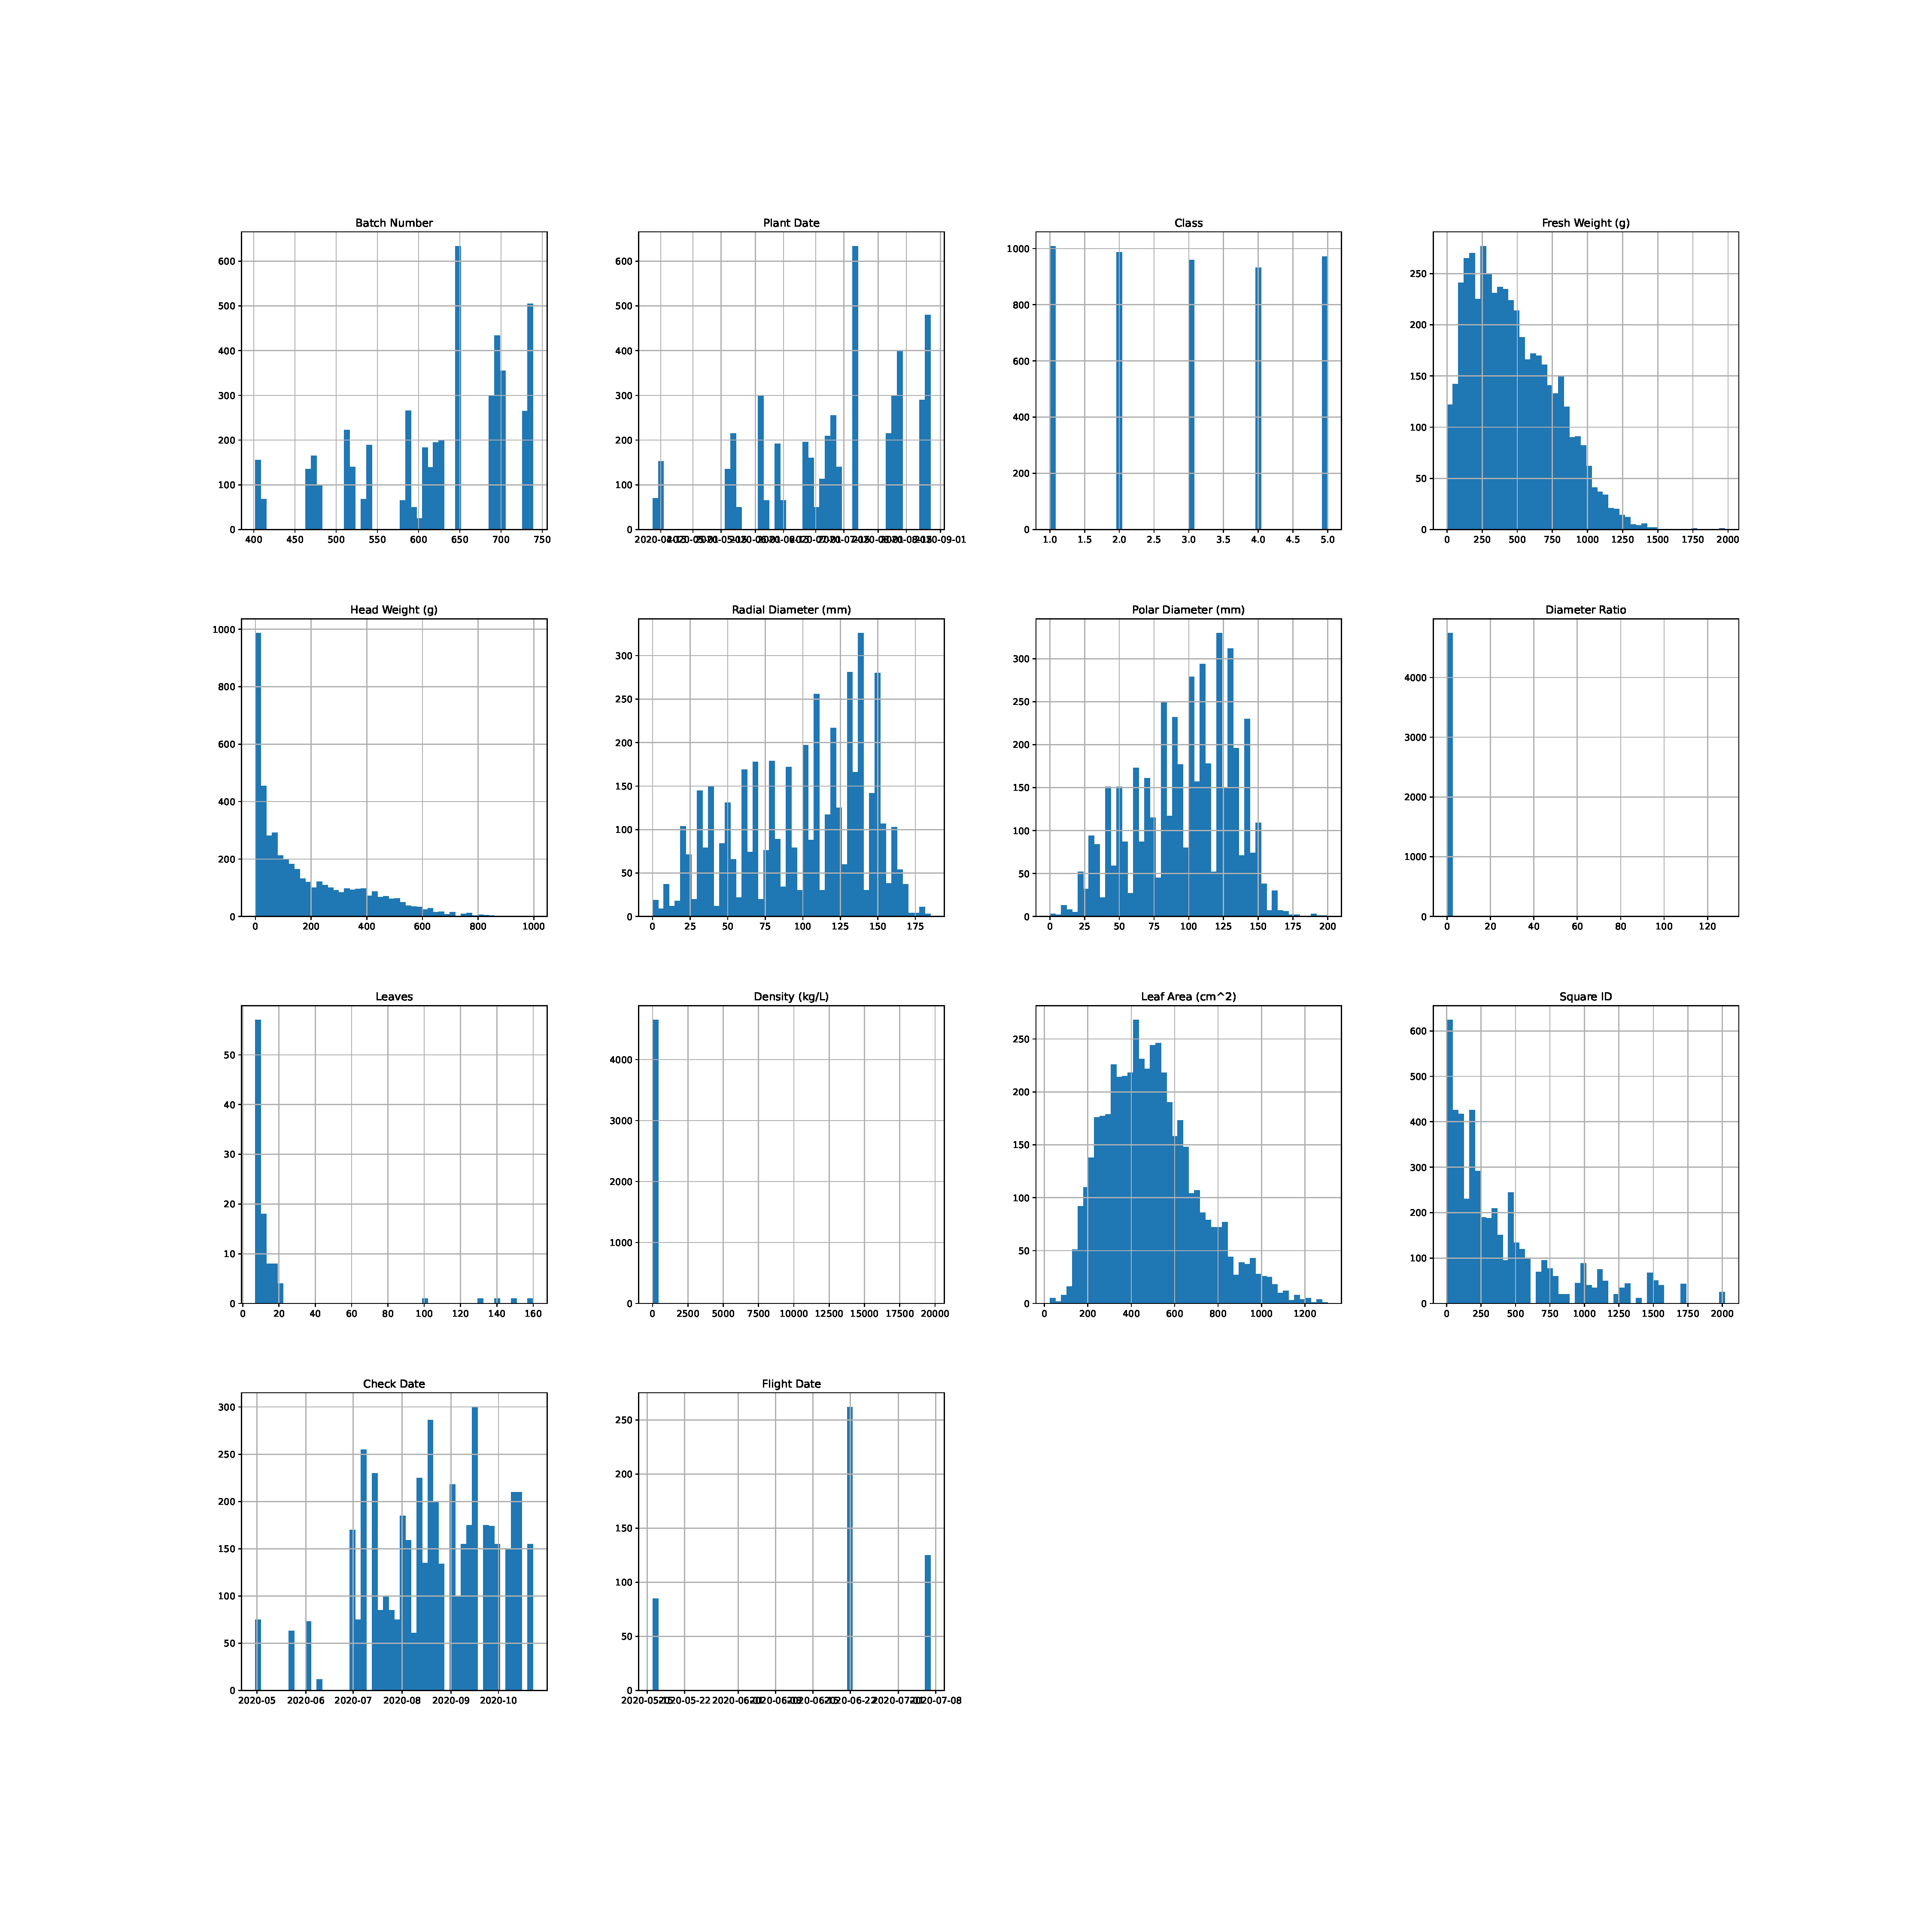
\includegraphics[width=0.7\textwidth]{plants_hist.pdf}
\caption{\label{fig:plants_hist}histogram plots of each column in plants dataframe.}
\end{figure}

Plants dataset has 4859 datapoints having various numeric and numpy datetime format. The weather dataset had 2556 datapoints with same varied variety of datatype as plants dataset. The numpy datetime format was first converted into pandas datetime format and was then split into day, month and year effectively converting numpy datetime type to int type.   

  

The remove column was handled by first dropping the corresponding rows for which the remove column was not empty. Then the entire column was dropped.  

  

Rows having plant date as nan or empty were dropped. New Datetime features were created such as the number of days from plant date to flight date were created. New day, month and year features were created from plant date, flight date and weather date.   

  

The weather dataframe contained some irrelevant data like battery voltage which doesn’t capture or convey any useful weather information and hence such columns were dropped. Other weather features like min and max of temperature, dew point and wind speed were removed however data having a summery statistic like average of these features was kept as they quantify the weather feature for that particular day more effectively. 

 

The target features range from 1.0 to 946.0 for Head Weigh, 10.0 to 178.0 for Polar Diameter and 10.0 to 185.0 for Radial Diameter. No scaling was applied to target features however scaling was used independently on each column without the influence of outliers. 




\section{Methodology}
After merging four separate dataframes into a single dataframe, the data was split into x and y where x are the merged features and y are the target features i.e. 'Head Weight (g)', 'Polar Diameter (mm)', 'Radial Diameter (mm)'. The train and target dataset was then created by taking the data points from x dataframe where the target features were not empty and corresponding data points from y as taken into target dataset. The target features along with 'Diameter Ratio', 'Density (kg/L)' were then dropped from train dataset 
After training set was created highly co related columns such as 'Dew\_Point\_Min', 'Batch Number', 'plant\_dates\_day', 'plant\_dates\_month' were dropped.
During model development train and target dataset was split into train and test datasets. 
Two sets of model evaluation and training was done, one with scaling and one without. As most of the models being trained were ensemble models scaling doesnt play a major role, however for support vector regressor and linear regressor (ie distance based models) the scale of the data does play a vital role as the distance is calculated based on the mean squared value of the input features.


 

\subsection{Baseline}
As R$^2$ and MSE metrics are used to determine the perfomance of the trained models, creating a baseline model will give a rough idea on how good or how bad a models' MSE score is. For baseline model a dummy estimator which predicts the mean was used. The model was trained on training set and the R$^2$ and MSE scores were calculated using the test split. No grid search or cross validation was performed for the dummy baseline estimator.\\
The results for baseline was:\\
MSE: 14628.058334157993 \\
R2: -0.0014616284462395008

\subsection{Model training}
For each of the above mentioned model a grid search for tuning the hyper parameters were performed. After getting the best performing parameters a new model with the best parameters was trained on the training dataset. The R$^2$ and MSE scores were calculated using the test split. While performing grid search a 10 fold cross validation was also performed to make sure the hyper parameters were tuned for generalizing over the dataset which also prevents overfitting.\\
The following are the chosen hyperparameters after gridsearch: \\\\
Support Vector Regressor: Best parameters: 'estimator\_\_C': 1000.0, 'estimator\_\_gamma': 3.511191734215127e-05\\ \\
AdaBoost Regressor: Best parameters: 'estimator\_\_learning\_rate': 0.5, 'estimator\_\_loss': 'linear', 'estimator\_\_n\_estimators': 60\\\\
Decision Tree Regressor: Best parameters: Best parameters:  'estimator\_\_max\_depth': 9, 'estimator\_\_min\_samples\_leaf': 9, 'estimator\_\_min\_samples\_split': 2\\\\
Voting Regressor: Meta estimators used: Random forest regressor, decision tree regressor and linear regressor\\No gridsearch was performed and default parameters were used for meta estimators and voting regressor


\section{Results}

The following are the results obtained:- \\\\
\begin{tabular}{llll}
Model                    & MSE         & R$^2$       & cross validation score \\
Support Vector Regressor & 1342.8742   & 0.87555  & 0.887504               \\
AdaBoostRegressor        & 1020.59812  & 0.90688  & 0.85922                \\
Voting Regressor         & 1224.9998   & 0.89662  & 0.91635                \\
DecisionTreeRegressor    & 1378.648286 & 0.89662  & 0.889732               \\
LinearRegression         & 2059.75915  & 0.813747 & 0.8511283             \\
\end{tabular}%
\\\\

The following are the results obtained after scaling the dataset:-\\
\begin{tabular}{llll}
Model                    & MSE        & R$^2$        & cross validation score \\
Support Vector Regressor & 1498.16201 & 0.87475   & 0.91114                \\
AdaBoostRegressor        & 1325.0069  & 0.863967  & 0.859109               \\
Voting Regressor         & 84341.8722 & -8.746842 & 0.917349               \\
DecisionTreeRegressor    & 1643.4975  & -8.74684  & 0.889718               \\
LinearRegression         & 771245.818 & -88.01964 & 0.8511283             
\end{tabular}


\section{Discussion}


From the above results it is clear that AdaBoost Regressor performed the best which has a higher R$^2$ and lower MSE score when compared to other models. It is also evident that scaling the dataset has negative impact on ensemble methods.
One reason maybe that the non linear relationships that was easily captured by the individual weak learners due to differences in the scale of the data was lost when the dataset was normalized. However SVR did perform better as it was expected to do when compared to unscaled dataset since its a distance based algorithm. A few improvements can be made such as creating a train, test and validation split instead of just train and test split. 
One advantage of using grid search with cross validation is that overfitting is reduced as the parameters are chosen for the given model while performing cross validation \cite{rodriguez2009sensitivity} and since at each step the cross validation scores are checked, parameters which overfit on training folds will not be chosen.

Another approach would be to improve the overall performance by using a more robust variant of adaboost regressor \cite{kummer2014adaboost}. Although over fitting problems were not observed here since a grid search with cross validation was performed to find the best parameters.
However if the dataset had many outliers or was bigger in size such that performing grid search would involve a lot of time and compute resources then overfitting would have occured and in such scenarios an implementation of adaboost which is robust to outliers and noise would be useful.
One limitation of this approach is that the weather features were just merged and fed into the model. If a more thorough feature engineering was performed on the weather dataset then some more useful data couldve been added to the final dataset which would in turn help the algorithm to model for more complex weather features. However modelling weather data is a complicated task on its own which requires deep domain expertise and using deep neural networks \cite{maqsood2004ensemble}.
Other statistical approaches like bootstrapping may not work in such a dataset where the number of features are high. 


\section{Conclusions}
As this project reflects a real world scenario very closely, developing a data driven solution would be very impactful. The adaboost model with unscaled dataset has achieved a low MSE and a high enough R$^2$ score. Further improvements include creating weather features. This includes creating a regressor for each of the columns and where the input will be lag features. Such a model would be used in predicting weather features for the dates in the year 2021.  

Another improvement would be to develop and train a LSTM for predicting weather features as its a time series dataset\cite{siami2019performance}. As modelling weather features is a complicated task using a non deep learning approach may not yield the required outcome. On the other hand as the dataset is limited in size feature engineering will play a vital role in modelling the weather data using deep learning approaches.

Another approach would be to use deep neural networks as neural networks are able to model the complex non linear relationships much more effectively than distance based machine learning models. As the dataset contains various weather and time features it would be a worthy effort to experiment with deep neural networks to predict the yield of crops\cite{bhojani2020wheat}.
As far as dataset is concerned, a much larger dataset would have been very useful in trying and experimenting with different models.


\bibliographystyle{abbrv}
\bibliography{sample}

\end{document}